%*******************************************************
%                       EINLEITUNG  
%*******************************************************
\chapter[Einleitung]{\label{sec:Einleitung}Einleitung}
% max 1 Seite
Mit den aktuellen Herausforderungen bei der Reduzierung von Treibhausgasen steigt das Interesse an Energiespeicherkonzepten, welche den Weg für energieeffiziente und nachhaltige Systeme ebnen. Besonders bei der Verwendung in mobilen Systemen, wie etwa elektrischen Fahrzeugen \cite{Huo2015,Donateo2015,Jochem2015,Kim2014,Orsi2016,Silva2011,Holdway2010,Sternberg2015,Ramachandran2015} und mobilen Robotern \cite{Hecht2023,Mikolajczyk2023,Ghobadpour2023,Wang2020}, haben sich die Vorteile von batteriebetriebenen Systemen gezeigt.

Herkömmliche Batterien sind oft nur wenig mechanisch belastbar, weshalb sie häufig mit einer zusätzlichen Schutzstruktur umgeben sind. Hinzukommt, dass durch die klare Funktionsteilung keine synergetischen Effekte genutzt werden können, wie z.B. bei Materialien, die sowohl als Energiespeicher als auch als Strukturkomponente dienen können. Das daraus resultierende niedrige Energiespeicher-zu-Masse-Verhältnis des Gesamtsystems ist eine der größten Schwächen dieser Technologie \cite{Armand2020,Schaefer2018,Cano2018,Goodenough2009}.
So nehmen die Materialien, die keinen Beitrag zur Energiespeicherung leisten, einen Massenanteil von etwa 40~\% in der von Audi Q4 e-tron Reihe eingebauten Batteriepacks ein \cite{Radu2021,Audi2022}, siehe Anhang~\ref{ch:AudiEnergie}. %Gesamtenergiedichte von 37~kWh/kg. Der Grenzwert für den Nutzen im Bereich des elektrischen Fliegens liegt nach \textsc{Scholz et al.} bei 51.8~Wh/kg \cite{Scholz2018}.

Ein vielversprechender Ansatz ist dabei die Entwicklung von sogenannten Struktur-Batterien, die zusätzlich zu ihrer Speicherfunktion auch lasttragend sein können \cite{Johannisson2018,Danzi2021,Wetzel2004, Thomas2004,Liu2009,Ekstedt2010,Wang2019,Asp2019, Moyer2020,Zhao2020, Yin2020,Wang2020,Lutkenhaus2020,Fu2021,Jin2021,Kalnaus2021,Wong2007,Carlson2013,Xu2022} und damit signifikante Einsparungen bei der Gesamtmasse und dem Gesamtvolumen ermöglichen \cite{Wetzel2004,Snyder2015,Carlstedt2020a,Asp2014,Johannisson2019}. Diese haben zudem den Vorteil, dass sie sich leichter in bestehende Designs integrieren lassen, was die Gewichtsverteilung erleichtern und einen Einbau näher am Verbraucher ermöglichen kann, wodurch Kabel eingespart werden. Diese Vorteile erlauben neue innovative Designs im Bereich Elektrofahrzeuge, elektrische Alltagsgeräte wie etwa Laptops und Telefone, mobile Roboter, Flugdrohnen und Satelliten.

Diese Dissertation fokussiert sich auf die computergestützte Suche von Struktur-Batterien in laminarer Bauweise.

Die hier dargestellte Forschung ist Teil der vom Deutschen Bundestag geförderten Forschungsinitiative „Luftfahrtforschung und -technologie“ LuFo-VI-2 in der Programmlinie „(A) Disruptive Technologien und innovative Systeme (ökoeffizientes Fliegen)“ im Fachbereich „(4) Strukturen und Bauweisen“ mit dem wichtigsten förderpolitischen Ziel „umweltfreundliche Luftfahrt“. Dies geschieht im Rahmen der „Entwicklung und Erprobung ultraleichter Verbundstrukturen mit integrierter elektrischer Speicherfunktion“ (ElViS).


%*************************************************************
%               Motivation und Zielstellung  
%*************************************************************
\section{\label{sec:Motivation_Zielstellung}Problemstellung und Zielsetzung}
% rund 1,5 Seiten inklusive Bild

%Um die Reichweite und Nutzungsdauer von mobilen elektrischen Geräten, wie Elektrofahrzeuge und mobile Roboter zu erhöhen ist sind elektrische Speicher mit besserem Verhältnis von Speichervermögen zu Gesamtmasse von entscheidenter Bedeutung. Aus dieser übergeordneten Zielstellung leiten sich drei mögliche Ansätze ab: erstens die Energiedichte der einzelnen Speicherzellen steigern, zweitens die Masse der mechansichen Entkoppelung durch die Verwendung von Werkstoffen mit hoher spezifischer Festigkeit und Steifigkeit reduzieren und drittens die Erhöhung der Gesamtenergiedichte durch die Verwendung von mechanisch belastbaren Batterien, welches einen Kompromiss zu den ersten beiden Ansätzten darstellt.

%Der letzte Ansatz hat außerdem den Vorteil, dass solche strukturtragenden Batterien (kurz Strukturbatterien) flexibler verbaut werden können und somit bei Verkabelung eingespart werden kann und Gewichtsverteilungsprobleme, wie sie etwa bei Flugmaschinen und Satelliten auftreten einfacher gelöst werden können

Derzeitige Strukturbatterien zeichnen sich oft durch eine große mechanische Steifigkeit und eine verhältnismäßig geringe Energiedichte aus. Dies macht sie jedoch für die meisten primären Anwendungsfälle ungeeignet und beschränkt damit ihr Anwendungsfeld auf sekundäre oder Schwachstromanwendungen (\textit{engl.} low energy applications). Der Mangel an Strukturspeichern mit signifkant höheren Energiedichten stellt neben noch weiteren ungeklären Fragestellungen zum Auswechseln und Recycling eine Markteintrittsbarriere da.

Hinzukommt, dass die bisherige Forschung in diesem Bereich sich hauptsächlich auf die Untersuchung und Verbesserung einzelner Komponenten wie Strukturelektrolyte und den Bau spezifischer Konfigurationen konzentriert. Dabei wurde jedoch eine ganzheitliche Methodik zur Verknüpfung der Erkenntnisse aus den verschiedenen Teilbereichen vernachlässigt. So lässt sich aktuell nur schwer bewerten, inwie weit in neues Material, was bessere Elektrochemische Eigenschaften, aber schlechtere mechanische Eigenschaften als ein beliebiges Referenzmaterial hat nun eher oder schlechter für den Einsatz in Strukturbatterien geeignet ist. Zudem basiert die Forschungsmethodik größtenteils auf experimentellen Ansätzen und wenigen computergestützten Modellen. Außerdem sind diese oft rechenintensiv und sind auf niedrigen Skalen auf den Einsatz von Supercomputern angewiesen. Des Weiteren benötigen die existierenden physikalischen Modelle eine Vielzahl an Materialkennwerten, die teilweise sehr aufwendig bestimmt werden müssen.

\begin{figure}[h]
	%\raggedleft
		%\def\svgwidth{\columnwidth}
        \center
	\includegraphics[width=\textwidth, angle=0]{motivation.pdf}
		\caption{\label{fig:motivation} Durch Strukturbatterien könnten a) eine Vielzahl an Anwendungen profitieren. Aktuelle Strukturbatterien zeigen jedoch noch viel ungenutztes Potenzial bei den elektrochemischen Eigenschaften, wie etwa Energiedichte.}
\end{figure}

Diese Dissertation zielt darauf ab, diese Lücke zu schließen durch die Entwicklung einer digitalen Methode. Diese soll dabei helfen den experimentellen Aufwand zu reduzieren und Neuerungen im wissenschaftlichen Bereich besser zu berücksichtigen und einzuschätzen. Dazu muss die Methodik in der Lage sein mit Daten sowohl aus der vorhandenen Literatur und eigenen Experimenten qualitative Aussagen über mögliche Stukturbatterievarianten zu einer Vielzahl an anwendungsgetriebenen Fragestellungen zu machen. 
Ausgangspunkt ist hierfür die Erarbeitung einer Modellgetrieben Auslegung mit eigener Erweiterung der Bewertung hinsichtlich fehlender Teilaspekte. Als erster Schritt dient hierbei die Erstellung einer Materialdatenbank für mögliche Strukturbatterienanwendungen. Dies beinhaltet auch die Recherche von Materialkandidaten aus dem Bereich Leichtbau und aktueller Batterieforschung. Die hierbei ermittelten Parameter dienen als Datengrundlage für Schritt zwei. In diesem werden exitierende computergestützten Modellen verknüpft und mit eigenen Modellen erweitert. Die eigenen Modelle werden mit Daten aus Literatur und Experimenten, die während des Projektzeitraums ElViS stattfanden einzeln validiert. Im dritten Schritt werden potenzielle Strukturspeicher mithilfe der validierten Einzelmodelle bewertet und exemplarisch an ausgewählten Kandidaten überprüft. Die ermittelten vorteilhaften Parameterkombinationen dienten \textsc{Kühn} und \textsc{Seidel-Greif} als Grundlage für ihre experimentellen Untersuchungen, die in einer prototypischen Fertigung einer Strukturbatterie kommulierte.

Mithilfe der entwickelten Methode konnte eine optimierte  Strukturbatterie für einen hybriden Anwendungsfall identifiziert werden und zeigte durch einen ersten Funktionsprototypen eine xx\% höhere multifunktionalen Performanz gegenüber bisher veröffentlichten Strukturbatterien.

% Das zugrundeliegende Prinzip dieses Lösungsansatzes besteht darin, dass Computer besser dazu geeignet sind, eine Vielzahl von einfachen Zusammenhängen zu verarbeiten und dies wiederholt für jede erdenkliche Kombination anzuwenden. Im Gegensatz zu bestehenden Ansätzen beginnt die Modellierung nicht auf atomarer Ebene, sondern auf der Komponentenebene, was eine schnellere Generierung von Ergebnissen ermöglicht. Zudem kann das Modellsystem leicht um Modelle auf mikro- oder molekularer Ebene erweitert werden, um zusätzliche Einflussfaktoren zu berücksichtigen.


%**************************************************************
%                   LITERATURÜBERSICHT  
%**************************************************************
\section{\label{sec:Literaturübersicht}Literaturübersicht}
% 3-5 Seiten

\subsection{Exitierende Strukturbatteriekonzepte}

\begin{figure}[h]
	%\raggedleft
		%\def\svgwidth{\columnwidth}
        \center
	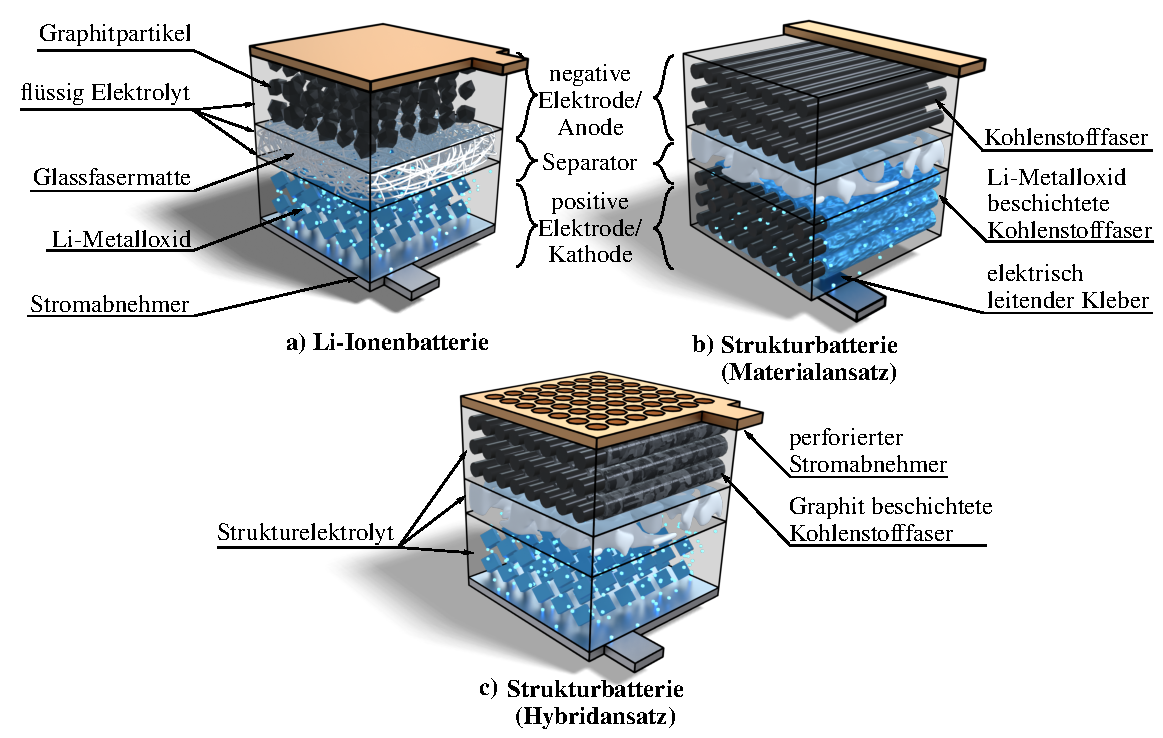
\includegraphics[width=\textwidth, angle=0]{sb_types.pdf}
		\caption{\label{fig:sb_types}Vereinfachte Darstellung von a) konventionellen Li-Ionen Batterie, b) einer Strukturbatterie als multifunktionales Material und c) als multifunktionale Struktur.}
\end{figure}

Die erste multifunktionale Strukturbatterie wurde 2004 von \textsc{Wetzel et al.} im Army Reasearch Laboratories (ARL) der USA entwickelt \cite{Wetzel2004, Snyder2006, Wong2007, Snyder2007}. Dieses Strukturbatterieverbundmaterial basierte auf Kohlenstofffasern als Anode und einer $\text{LiFePO}_\text{4}$ beschichteten Edelstahlkathode und eine Glasfasermatte als Separator \cite{Wong2007}. Dieser Aufbau zeigte bereits gute mechanische Eigenschaften. Allerdings konnten die elektrochemischen Eigenschaften wegen auftretenden Kurzschlüssen nicht final bestimmt werden.

2009 konzeptionierte \textsc{Liu et al.} \cite{Liu2009} die erste Kurzfaserverträrkte Elektrode mit einem festen Polymerelektrolyte als Matrixmaterial. Allerdings konnte das Team die faserverstärkte Elektrode herstellen oder einen Feststoffelektrolyte mit ausreichender Ionenleitfähigkeit finden, weshalb schließlich auf ein Gelbasiertes Elektorlyte, mit festem und flüssigen Phasenanteil umgeschwenkt wurde. Da aufgrund der besseren Ionenleitfähigkeit weniger des Elektrolytes eingesetzt werden musste konnte eine Energiedichte von 35~Wh/kg erreicht werden.  Durch die fehlende strukturelle Verstärkung wurden allerdings nur eine verhältnismäßig geringe Zugsteifigkeit von 3 GPa erreciht werden.

Der Ansatz des Gelelektrolyten wurde von \textsc{Ekstedt et al.} aufgenommen \cite{Ekstedt2010}, der erstmalig in diesen ein Kohlenstofffasergewebe einbettete. Ähnlich zu den Arbeiten von \textsc{Wetzel et al.} wurde auch hier auf einen Glasfaser basierten Separator und eine $\text{LiFePO}_\text{4}$ beschichte gewebte Aluminiumfasermatte als Kathode. Die resultierende Batterie zeichnete sich durch eine Zellspannung von 3,3~V aus. Jedoch wurden die mechanischen und elektrochemischen Eigenschaften nur theoretisch ermittelt.

Im Jahr 2011 \textsc{Carlson et al.} \cite{Carlson2011} eine der ersten funktionierenden Strukturbatterien mit einer laminatartartigen Struktur, die sich aus einem IMS65 Kohlenstofffaserngebe als Anode, einem Gelelektrolyte, Glasfaserseparator und einer  $\text{LiFePO}_\text{4}$ beschichte gewebte Aluminumfolie. Die speicherbare elektroische Energie betrug 0,0247~Wh/kg, was  was ausreichend war um eine LED 70~s lang zum glimmen zu bekommen.

Zwie Jahr später wurden \textsc{Asp et al.} \cite{Asp2013US,Asp2013CN} zwei Patentente zugesprochen, welches einen Ansatz der durch gezielte funktionailiserung der Faseroberflächen, jede Kohlenstofffaser zu einer Elektrode macht. Auch wenn die Patente seit 2017 nicht mehr verfolgt werden, konnte mittels aufbauend wurde eine Batterie mit 
Dadurch wurden eine Energiedichte 10~Wh/kg erzielt, die theortisch möglichen 175 Wh/kg bei einem gleichzeitigen Schubmodul von 1 GPa, wurden jedoch noch noch nicht ansatzweise erreicht \cite{Leijonmarck2013, Carlson2013}.

2018 untersuchte \textsc{Meng et al.} \cite{Meng2018} erstmalig den Einsatz von vertiakl ausgerichten Karbonnanoröhren (CNT), diese wurden für die Elktrode auf ein Edelstahlnetz aufgedampft. Anschließedn wurde für die Anode $\text{NiO}_\text{x}$ durch einen elektroschemischen Ausscheideprozess eingelagert. Mit dem gleichen Verfahren wurde mit $\text{FeO}_\text{x}$ für die Kathode auf die CNT-Edelstahlelektrode eingelagert. Die Strukurbatterie erreichte dabei eine Zugsteifigkeit von 7,0~GPa und eine Energiedichte von 1.4~Wh/kg.

\textsc{Moyer et al.} \cite{Moyer2020} Gruppe modifizierte den für Patterientypischen Pouchzellenansatz in dem das verpresste Kohlenstoffasergewebe als Stromkolletor und Schutzfolie dient. Durch das anodenseitige Aufbringen von Graphit und $\text{LiFePO}_\text{4}$ auf der Kathode nehmen die Fasern aber nicht direkt am chemischen Prozess teil. Durch das bessere Interkalationsverhalten bei Graphit konnte aber eine hohe Energiedichte von 35~Wh/kg gemessen werden. Jedoch führte der Ansatz zu einer vergleichweise geringen Zugsteifigkeit von 2~GPa.

\textsc{Thakur et Dong} \cite{Thakur2020} stellten 2020 die erste 3D gedruckte Strukturbatterie her. Mithilfe eines Koextrusionsprozesses konnte eine Kohlenstofffaser die vorher mit einem festen Polymerelktrolyte beschichtet wurde, zusammen mit einem Li gedopted Matrixmaterial aufgepracht werden. Nachdem Drukcen der Elektrode wurde manuel eine Glasfasermatte und abschließend eine Alumiumfolie als Gegenelektrode aufgebracht. Neben der Möglichkeit neue Batterieformen zu drucken wurde auch durch die höhere Dichte an Aktivmaterial in Fasernähe eine vergleichweise hohe Energiedichte von 24~Wh/kg erreicht. Allerdings konnte durch den geringen Faservolumenanteil ein geringes Zugmodul von 0.29~GPa gemessen werden.

2021 präsentierte \textsc{Asp et al.} \cite{Asp2021} ein Design mit unidirectionalen Kohlenstofffasern als Anode, einem gewebbten Glassfaserseparator und einer $\text{LiFePO}_\text{4}$ beschichteten Aluminiumplatte als Kathode. Durch ein verbessertes Herstellungsverfahren und eine günstige Faseranordnung konnte eine Zugsteifigkeit von 25~GPa und Zugfestigkeit von 300~MPa gemessen werden. Gleichzeitig erreichte die Strukturbatterie 24~Wh/kg. \textsc{Siraj et al.} \cite{Siraj2023} verbesserten zwei Jahre später den Infiltrationsprozess um bei annährend gleichbleibenden mechanischen Eigenschaften die Energiedichte auf 41~Wh/kg nahezu zuverdoppeln.

\begin{table}[ht]
    \centering
    \caption{Übersicht bisher entwickelter Strukturbatterien.}
    \begin{tabular}[t]{lccc}
    \toprule
    &Zugmodul~[GPa]&Energiedichte~[Wh/kg]&Referenz\\
    \midrule
    \textsc{Wong et al.}&8&/&\cite{Wong2007}\\
    \textsc{Liu et al.}&3&35& \cite{Liu2009}\\
    \textsc{Meng et al.}&7&4&\cite{Meng2018}\\
    \textsc{Moyer et al.}&35&2&\cite{Moyer2020}\\
    \textsc{Thakur et Dong}&0.29&24&\cite{Thakur2020}\\
    \textsc{Huang et al.}&9.2&43&\cite{Huang2020}\\
    \textsc{Asp et al.}&25&24&\cite{Asp2021} \\
    \textsc{Saraj et al.}&26&41&\cite{Siraj2023}\\
    \bottomrule
    \end{tabular}
\end{table}%

Die exitierenden Studien an Strukturbatterieverbundmaterialien zeigen eine reihe an Verbesserungspotenzialen für weitere Forschungen. Die größte Herausforderung stellt dabei das Erzielen einer möglichst guten Lithiuminterkalation in das Aktivmaterial der Elektrode und unbehinderten Lithiummigration zwischen diesen, bei gelichzeitiger Beibehaltung der mechanischen Steifigkeit und Festigkeit \cite{Asp2015}.
Auch ist die aktuell höchste erreichte Energiedichte von 35~Wh/kg am unteren Ende der benötigten Energiedichte, die für den Einsatz in z.B. Elektrofahrzeugen benötigt wird. Diese minimale Einstiegsgrenze wurde allerding 2022 von dem Forschungsteam von \textsc{Linde} am Deutschen Luft und Raumfahrtzentrum (DLR) weiter angehoben und befindet sich eher bei einer Energiedichte von 74~Wh/kg mit einem Zugmodul und -festigkeit von 54~GPa bzw. 203 MPa und einer Leistungsdichte von 376~W/kg \cite{Ishfaq2022}.

\subsection{Beschreibung des elektrochemischen und mechanischen Verhaltens von Strukturbatterien}
Einer der größten Herausforderungen ist bei der Entwicklung von neuen Strukturbatterien besteht in der Beachtung aller auftretenden Wechselwirkungen, die durch den hohen Multifunktionalitätsgrad in Material und Struktur zustande kommen.

Eine verhältnismäßig simple Beschreibung der elektrochemischen und thermischen Prozesse kann durch äquivalente Ersatzschaltungen (\textit{engl.} equivalent circuit model) (ECM) erfolgen \cite{Bavsic2022}. Bereits mit wenigen Elementen lassen sich Spannungsänderungen in Abhängigkeit zum Aufund Entladeverhalten gut annähern \cite{YannLiaw2004}. Durch zusätzliche Erweiterungen lassen sich auch Alterung und der Einfluss zahlreicher thermischer Effekte berücksichtigen\cite{Hannan2017,Tran2021}.
Durch den geringen Rechenaufwand eigenen sich diese Modelle sehr gut für zeitkristische Anwendungen wie etwa zur Lade- und Entladeregelung. Die Modellparameter müssen jedoch jedes Mal erst durch einen Fittingprozess für das jeweilige System bestimmt werden \cite{Tomasov2019}. Eine Verbindung der einzelnen Schaltelemente mit real-physikalischen Größen hatte bisher nur wenig erfolg \cite{Plett2015}.

Die pyhiskalische Modellierung der elektrochemischen Prozesse wurde maßgeblich von \textsc{Doyle}\cite{Doyle1995,Doyle2003,Ceder2002}, \textsc{Fuller}\cite{Fuller2018,Takeuchi2008} und \textsc{Newman}\cite{Doyle1995,Newman2021} vorran gebracht. Das von ihnen entwickelte und nach ihnen benannte DFN Modell (alternativ auch \textit{pseudo zwei dimensionale} (P2D) Modell bezeichnet) \cite{Doyle1993} beschreibt die Prozesse auf der Markroskala und eigenet sich somit sehr um die Vorgänge auf Zellebene zu modellieren. Die benötigten Parameter können durch Experimente oder mit hilfe von Simulationen auf niedrigeren Skalen, wie etwa Dichtefunktionaltheorie (DFT) oder Molekül dynamisiche (MD) Simulationen bestimmt werden \cite{Chen2022}. Das DFN-Modell findet heute weitreichenden Einsatz und erfuhr seit seiner Veröffentlichung 1993 zahlreiche Modifikationen und Erweiterungen. Eine paar der bekanntesten Derivate sind dabei das \textit{Single Particle Model} (SPM) \cite{Li2017} von \textit{full homogenized macro-scale} (FHM) Modell \cite{Arunachalam2019}, welche beide darauf abzielen die sehr rechenaufwendigen Differentialgleichungen in ihrer Komplexität zu reduzieren. 

Mit der Kopplung der thermischen Prozessen wurde bereits 1995 von \textsc{Pals et Newman} \cite{Pals1995,Pals1995a} begonnen und seit dem stetig weiterausgebaut \cite{Chen2005,Onda2006,Kim2013,Gao2021,Liu2023}. Auch der Einfluss von lithierungsbedingter Ausdehung 
\cite{Bower2011,Yang2014,Roberts2014,Pereira2019,Mai2019,Li2020,Hoeschele2023}, Rissbildung \cite{Dionisi2017,Wang2020a,Pistorio2023} und Alterung \cite{RedondoIglesias2020} wurden in vielzähligen Studien untersucht. Zusätzlich existieren bereits viele Studien, die sich an einer vereinheitlichten Modellierung aller Effekte \cite{Wu2014,Kim2018,Liu2020,Yin2020} und auch über mehrere Größenskalen versuchen \cite{Liu2019,Li2020a,Katrasnik2021}.

\textsc{Carlsted} erarbeitete Stückweise in einer Reihe von Beiträgen eine Koppelung von Elektrochemie, Mechanik und Thermodynamik um das Verhalten von Strukturbatterien zu beschreiben \cite{Carlstedt2019,Carlstedt2019a,Carlstedt2019b,Carlstedt2020,Carlstedt2020b, Carlstedt2022,Carlstedt2022a,Carlstedt2022b}. Auch wurde der Ansatz um den nicht-lineare Zusammenhang durch die Gestaltänderung von \textsc{Larsson et al.} \cite{Larsson2023} erweitert. 

\subsection{Modellierungsgetriebene Entwicklung von neuen Batterien und Strukturbatterien}

Die neu-motivierte Forschung in bereits untersuchte und neue Batteriematerialien baut aktuell hauptsächlich auf theoretischen Vorüberlegungen und experimentellen Prototypen auf. Um die Vielzahl an Effekten zu berücksichtigen und der enormen Anzahl an vielversprechenden Materialkombinationen herzuwerden argumentierten \textsc{Greenhalgh} \cite{Greenhalgh2024,Greenhalgh2024a} und \textsc{Asp} \cite{Asp2024} auf dem \textsc{1st Structrual Power Research Showcase} in London, dass nur durch eine intensive Modellierungsarbeit diese Varianten voruntersucht und genügend eingeschränkt werden können.
Der multiphysikalische Modellierungsansatz von \textsc{Carlsted} wird zwar in diesmen Zusammenhang oft erwähnt, allerdings sorgen Skalierungseffekte, wei etw Defekte und Faser-Matrix-Interfaceeffekte, die besonders bei Oberflächenmodifikation von Kohlenstofffasern sowohl für deutlich andere elektroschemische und mechansiche Eigenschaften des Verbundes sorgt, für große Ungenauigkeiten bei der Adaption \cite{Franco2019,Fam2024}. Hinzukommt, dass die Modelle von Carlsed mit zunehmender Komplexität immer mehr Materialparameter benötigen und bereits jetzt mehr als 20 teils aufwendig zu bestimmende Parameter pro Material benötigen \cite{Greenhalgh2024a}. Bis heute wurde dieser Ansatz daher vorallem zur nachträglichen Validierung und zur detallierten Untersuchung von sensorische und aktuatorischen Effekten von Strukturbatterien benutzt \cite{Carlstedt2023}.

Die einzige zur Zeit exitierende Veröffentlichung zur Vorhersage von Energiedichte und Zugsteifigkeit ist zwar ebenfalls von \textsc{Carlsted}\cite{Carlstedt2018}. Jedoch wurden dazu ein in der Komplexität deutlich reduzierter Ansatz benutzt. Hinzukommt, dass bei der Auswertung nur drei Varianten untersucht wurden, die sich ihren Elektrodendicke und dem Volumenanteil des Aktivmaterial unterschieden. Außerdem wurde der Einfluss des Elektrolytes nicht berücksichtigt.








% Dan Zenkert KTH Prof (Fasercehmie), 
% Dr Faye Smith OBE (Director at Avalon Consultancy Services)
% Peter Linde (DLR, CORCER Mitgleid)
% Milo Shaffer ( Professor of Materials Chemistry London)
% Natasha Shirshova (Lecturer in Engineering Materials at Durham University)
% Derrick Fam (Scientist at Institute of Materials Research and Engineering (IMRE), Adjunct Assistant Professor (NTU, MSE), Dy. Dir. Singapore Battery Consortium)
% Alexander Bismarck (Professor of Material Chemistry Wien)
% Madhavi Srinivasan (Professor at Nanyang Technological University Singapore)



   

